% mnras_guide.tex
%
% MNRAS LaTeX user guide
%
% v3.0 released 22 May 2015
% (version numbers match those of mnras.cls)
%
% Copyright (C) Royal Astronomical Society 2015
% Authors:
% Keith T. Smith (Royal Astronomical Society)

% Change log
%
% v3.0   September 2013 - May 2015
% * <buder@mpia.de> 2017-10-27T05:54:29.871Z:
%
% ^.
%    First version: complete rewrite of the user guide
%    Basic structure taken from mnras_template.tex by the same author

%%%%%%%%%%%%%%%%%%%%%%%%%%%%%%%%%%%%%%%%%%%%%%%%%%
% Basic setup. Most papers should leave these options alone.
\documentclass[fleqn,usenatbib,useAMS]{mnras}

%%%%% AUTHORS - PLACE YOUR OWN PACKAGES HERE %%%%%

% Only include extra packages if you really need them. Common packages are:
\usepackage{graphicx}	% Including figure files
\usepackage{amsmath}	% Advanced maths commands
\usepackage{amssymb}	% Extra maths symbols
\usepackage{multicol}        % Multi-column entries in tables
\usepackage{bm}		% Bold maths symbols, including upright Greek
\usepackage{pdflscape}	% Landscape pages
\usepackage{enumitem}	% Including figure files
\usepackage{multirow}   % Allow multi-row cells in tables
\usepackage{CJK}
\usepackage{longtable}

%this fixes the problem of when hyperref links are broken over two pages.
\usepackage{etoolbox}
\makeatletter
\patchcmd\@combinedblfloats{\box\@outputbox}{\unvbox\@outputbox}{}{%
   \errmessage{\noexpand\@combinedblfloats could not be patched}%
}%
 \makeatother
%%%%%%%%%%%%%%%%%%%%%%%%%%%%%%%%%%%%%%%%%%%%%%%%%%

%%%%%% AUTHORS - PLACE YOUR OWN MACROS HERE %%%%%%

%%%%%%%%%%%%%%%%%%%%%%%%%%%%%%%%%%%%%%%%%%%%%%%%%%

% Use vector fonts, so it zooms properly in on-screen viewing software
% Don't change these lines unless you know what you are doing
\usepackage[T1]{fontenc}
\usepackage{ae,aecompl}

% MNRAS is set in Times font. If you don't have this installed (most LaTeX
% installations will be fine) or prefer the old Computer Modern fonts, comment
% out the following line
\usepackage{newtxtext,newtxmath}
% Depending on your LaTeX fonts installation, you might get better results with one of these:
%\usepackage{mathptmx}
%\usepackage{txfonts}

%@arxiver{galah_rzxy_bstep.pdf, DR2_example_spectra.pdf, Abundance_overview_flag_0_snr_0.pdf}

\begin{document}
\begin{CJK*}{UTF8}{gbsn}
\label{firstpage}
\pagerange{\pageref{firstpage}--\pageref{lastpage}}

%%%%%%%%%%%%%%%%%%% TITLE PAGE %%%%%%%%%%%%%%%%%%%

% Title of the paper, and the short title which is used in the headers.
% Keep the title short and informative.
\title{The GALAH Survey: Third Data Release}

% The list of authors, and the short list which is used in the headers.
% If you need two or more lines of authors, add an extra line using \newauthor
\author[Buder et al.]{Sven Buder$^{1,2}$\thanks{Contact e-mail: \href{mailto:buder@mpia.de}{buder@mpia.de}},
and~the~GALAH~collaboration
\\
\\
$^{1}$Max Planck Institute  for Astronomy (MPIA), Koenigstuhl 17, 69117 Heidelberg, Germany\\
$^{2}$Fellow of the International Max Planck Research School for Astronomy \& Cosmic Physics at the University of Heidelberg, Germany
%(Affiliations listed after the references)
}

% These dates will be filled out by the publisher
\date{Accepted 2019 MM DD. Received 2019 MM DD}

% Enter the current year, for the copyright statements etc.
\pubyear{2019}

% Don't change these lines
\maketitle
\end{CJK*}

% Abstract of the paper
\begin{abstract}
The GALAH survey has continued observations and data analysis after its second Data Release in April 2018. After this Data Release, the \textit{Gaia} collaboration has also released their second data set with an overlap of XX\% with the stars observed by GALAH. The exquisite parallax information delivered with \textit{Gaia} DR2 has allowed the GALAH collaboration to adjust the data analysis for all stars in order to take this astrometric data and photometry from 2MASS into account when optimising the stellar spectroscopic parameters.
In this paper we explain the new analysis pipeline in detail and present the validation tests performed for the data published as part of GALAH Data Release 3.
\end{abstract}

% Select between one and six entries from the list of approved keywords.
% Don't make up new ones.
\begin{keywords}
Surveys -- 
the Galaxy --
methods: observational --
methods: data analysis --
stars: fundamental parameters -- 
stars: abundances
\end{keywords}

%%%%%%%%%%%%%%%%%%%%%%%%%%%%%%%%%%%%%%%%%%%%%%%%%%

%%%%%%%%%%%%%%%%% BODY OF PAPER %%%%%%%%%%%%%%%%%%

%\newpage
%________________________________________________________________
\section{Introduction} \label{sec:introduction}

%\newpage
%________________________________________________________________
\section{Target selection, observation, reduction} \label{sec:selection_observation_reduction}

\subsection{Target selection}\label{sec:target_selection}

\subsection{Observations}\label{sec:observation}
    
\subsection{Data reduction}\label{sec:reduction}


%\newpage
%________________________________________________________________
\section{Analysis} \label{sec:analysis}

\subsection{Analysis strategy} \label{sec:analysis_strategy}

We have run SME on the full survey data
 
\subsection{Analysis step 1: Stellar parameters for the whole sample with \textit{Spectroscopy Made Easy}} \label{sec:analysis_step1}



\begin{figure*}
  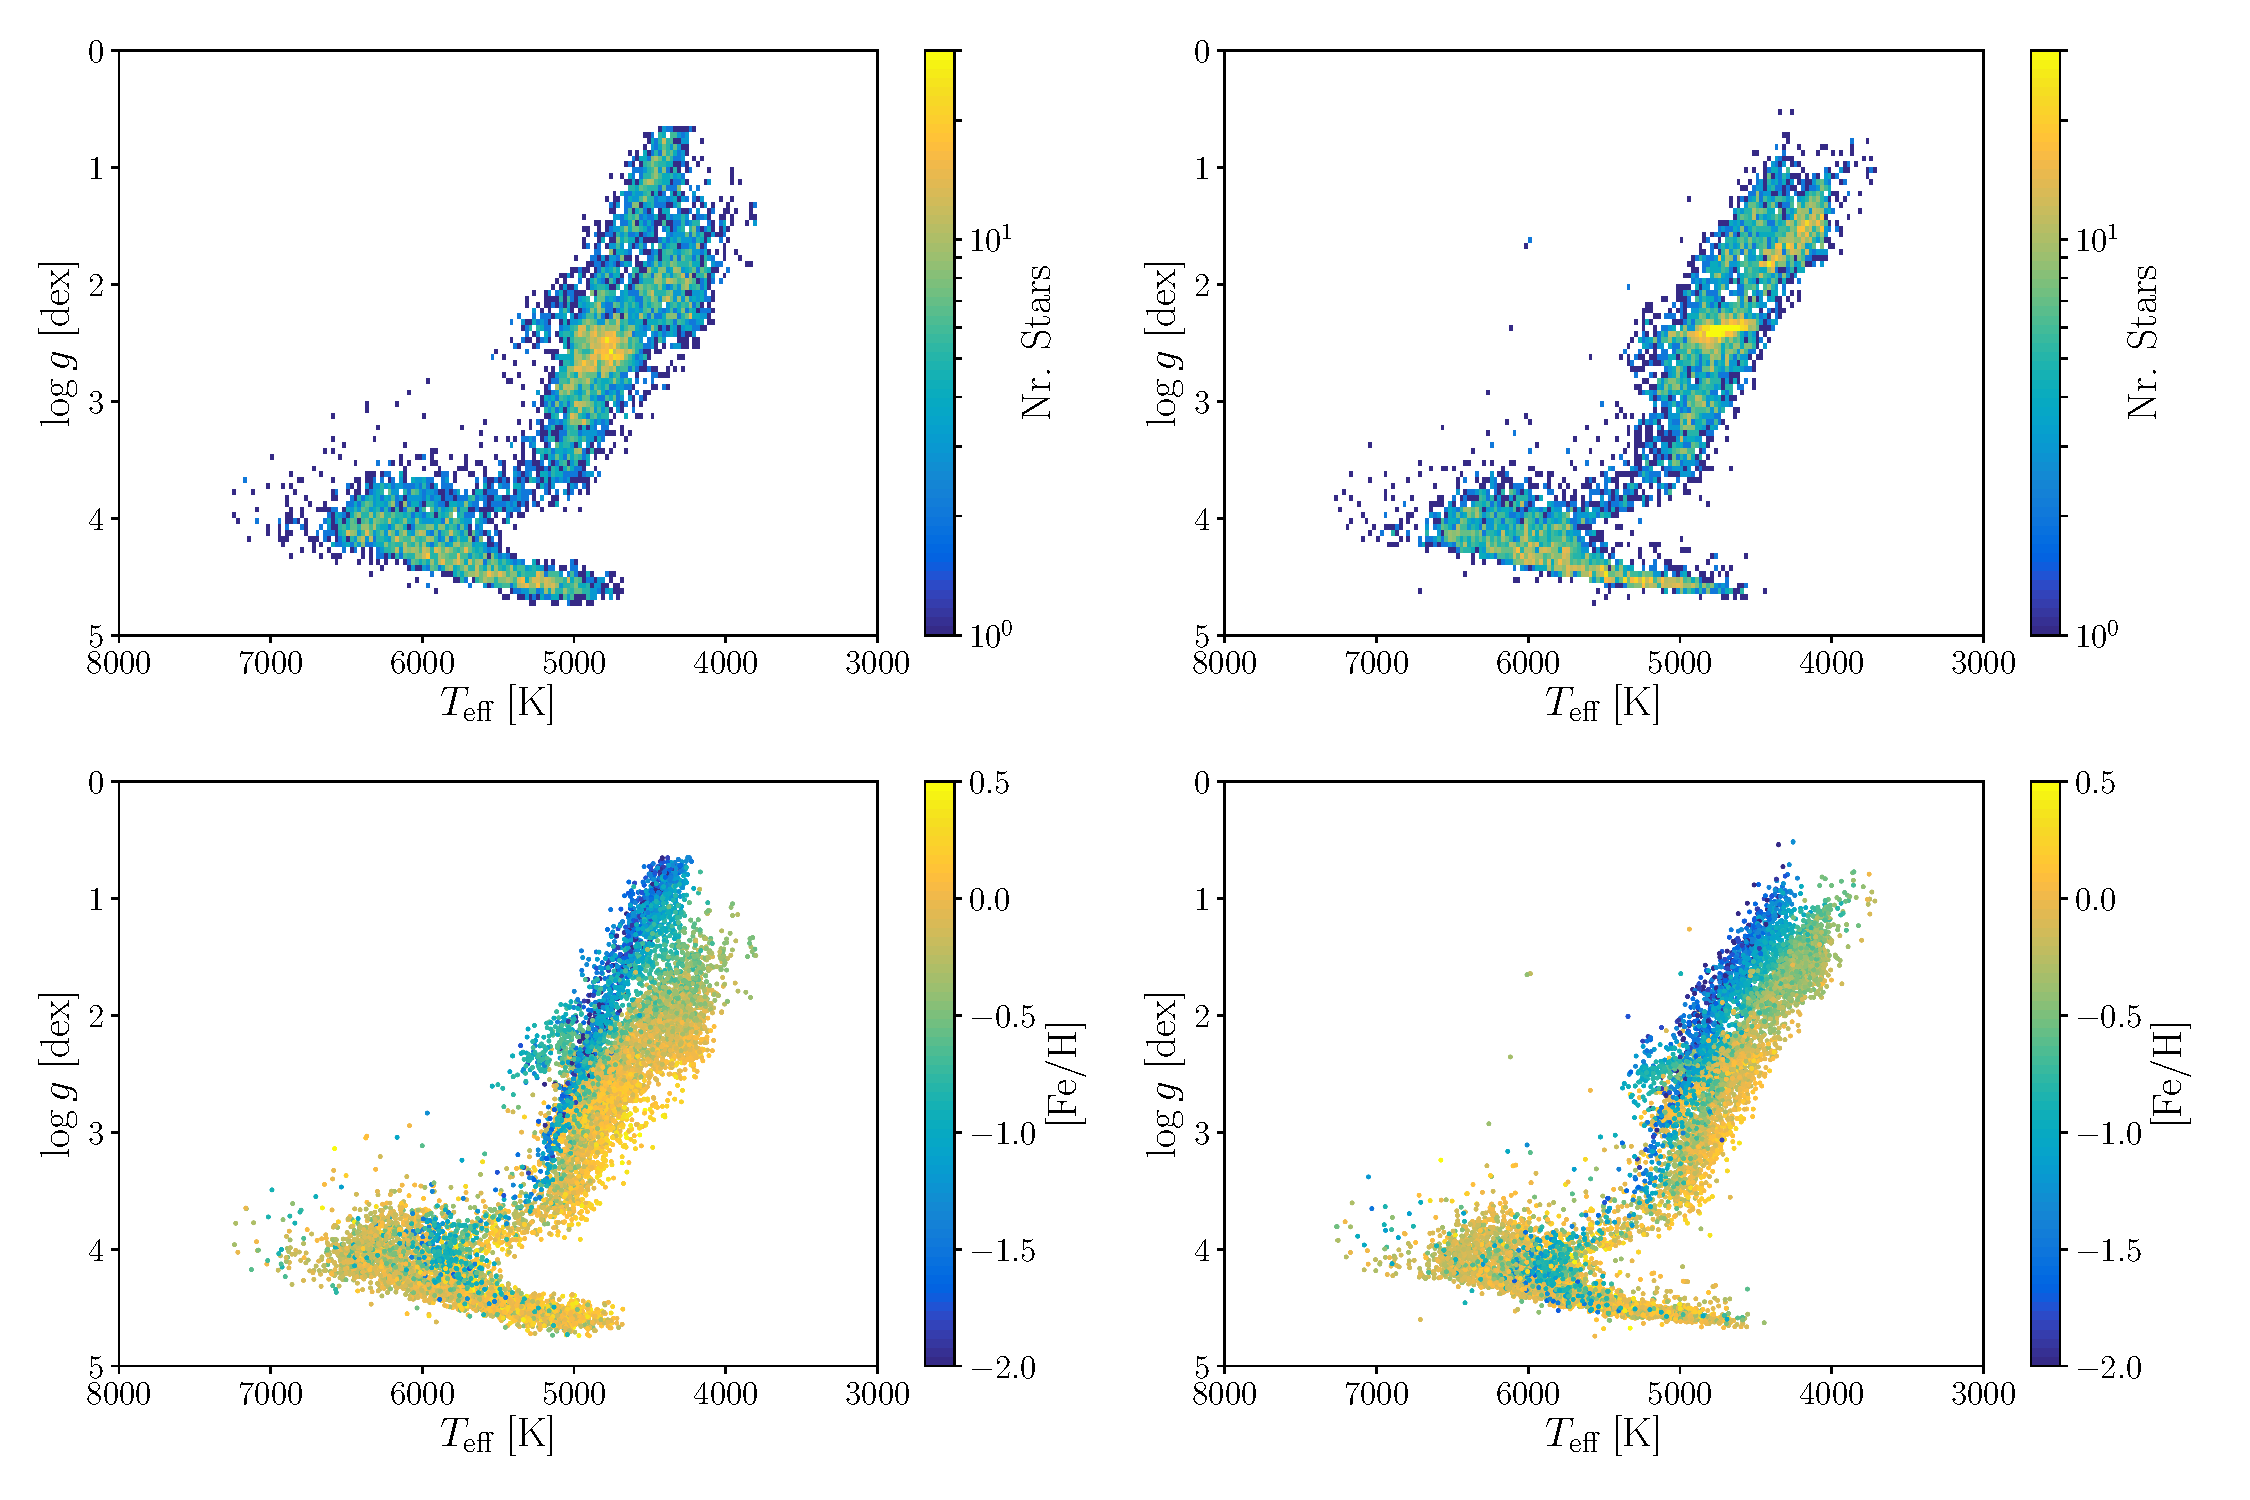
\includegraphics[width=\textwidth]{{Figures/dr2_rerun_kiel_comparison}.pdf}
  \caption{Caption} 
  \label{fig:dr2_rerun_kiel_comparison}
\end{figure*}

\subsection{Analysis step 2: Validation and flagging of stellar parameters} \label{sec:analysis_step1}

\subsubsection{\textit{Gaia} FGK benchmark stars}

\begin{figure*}
  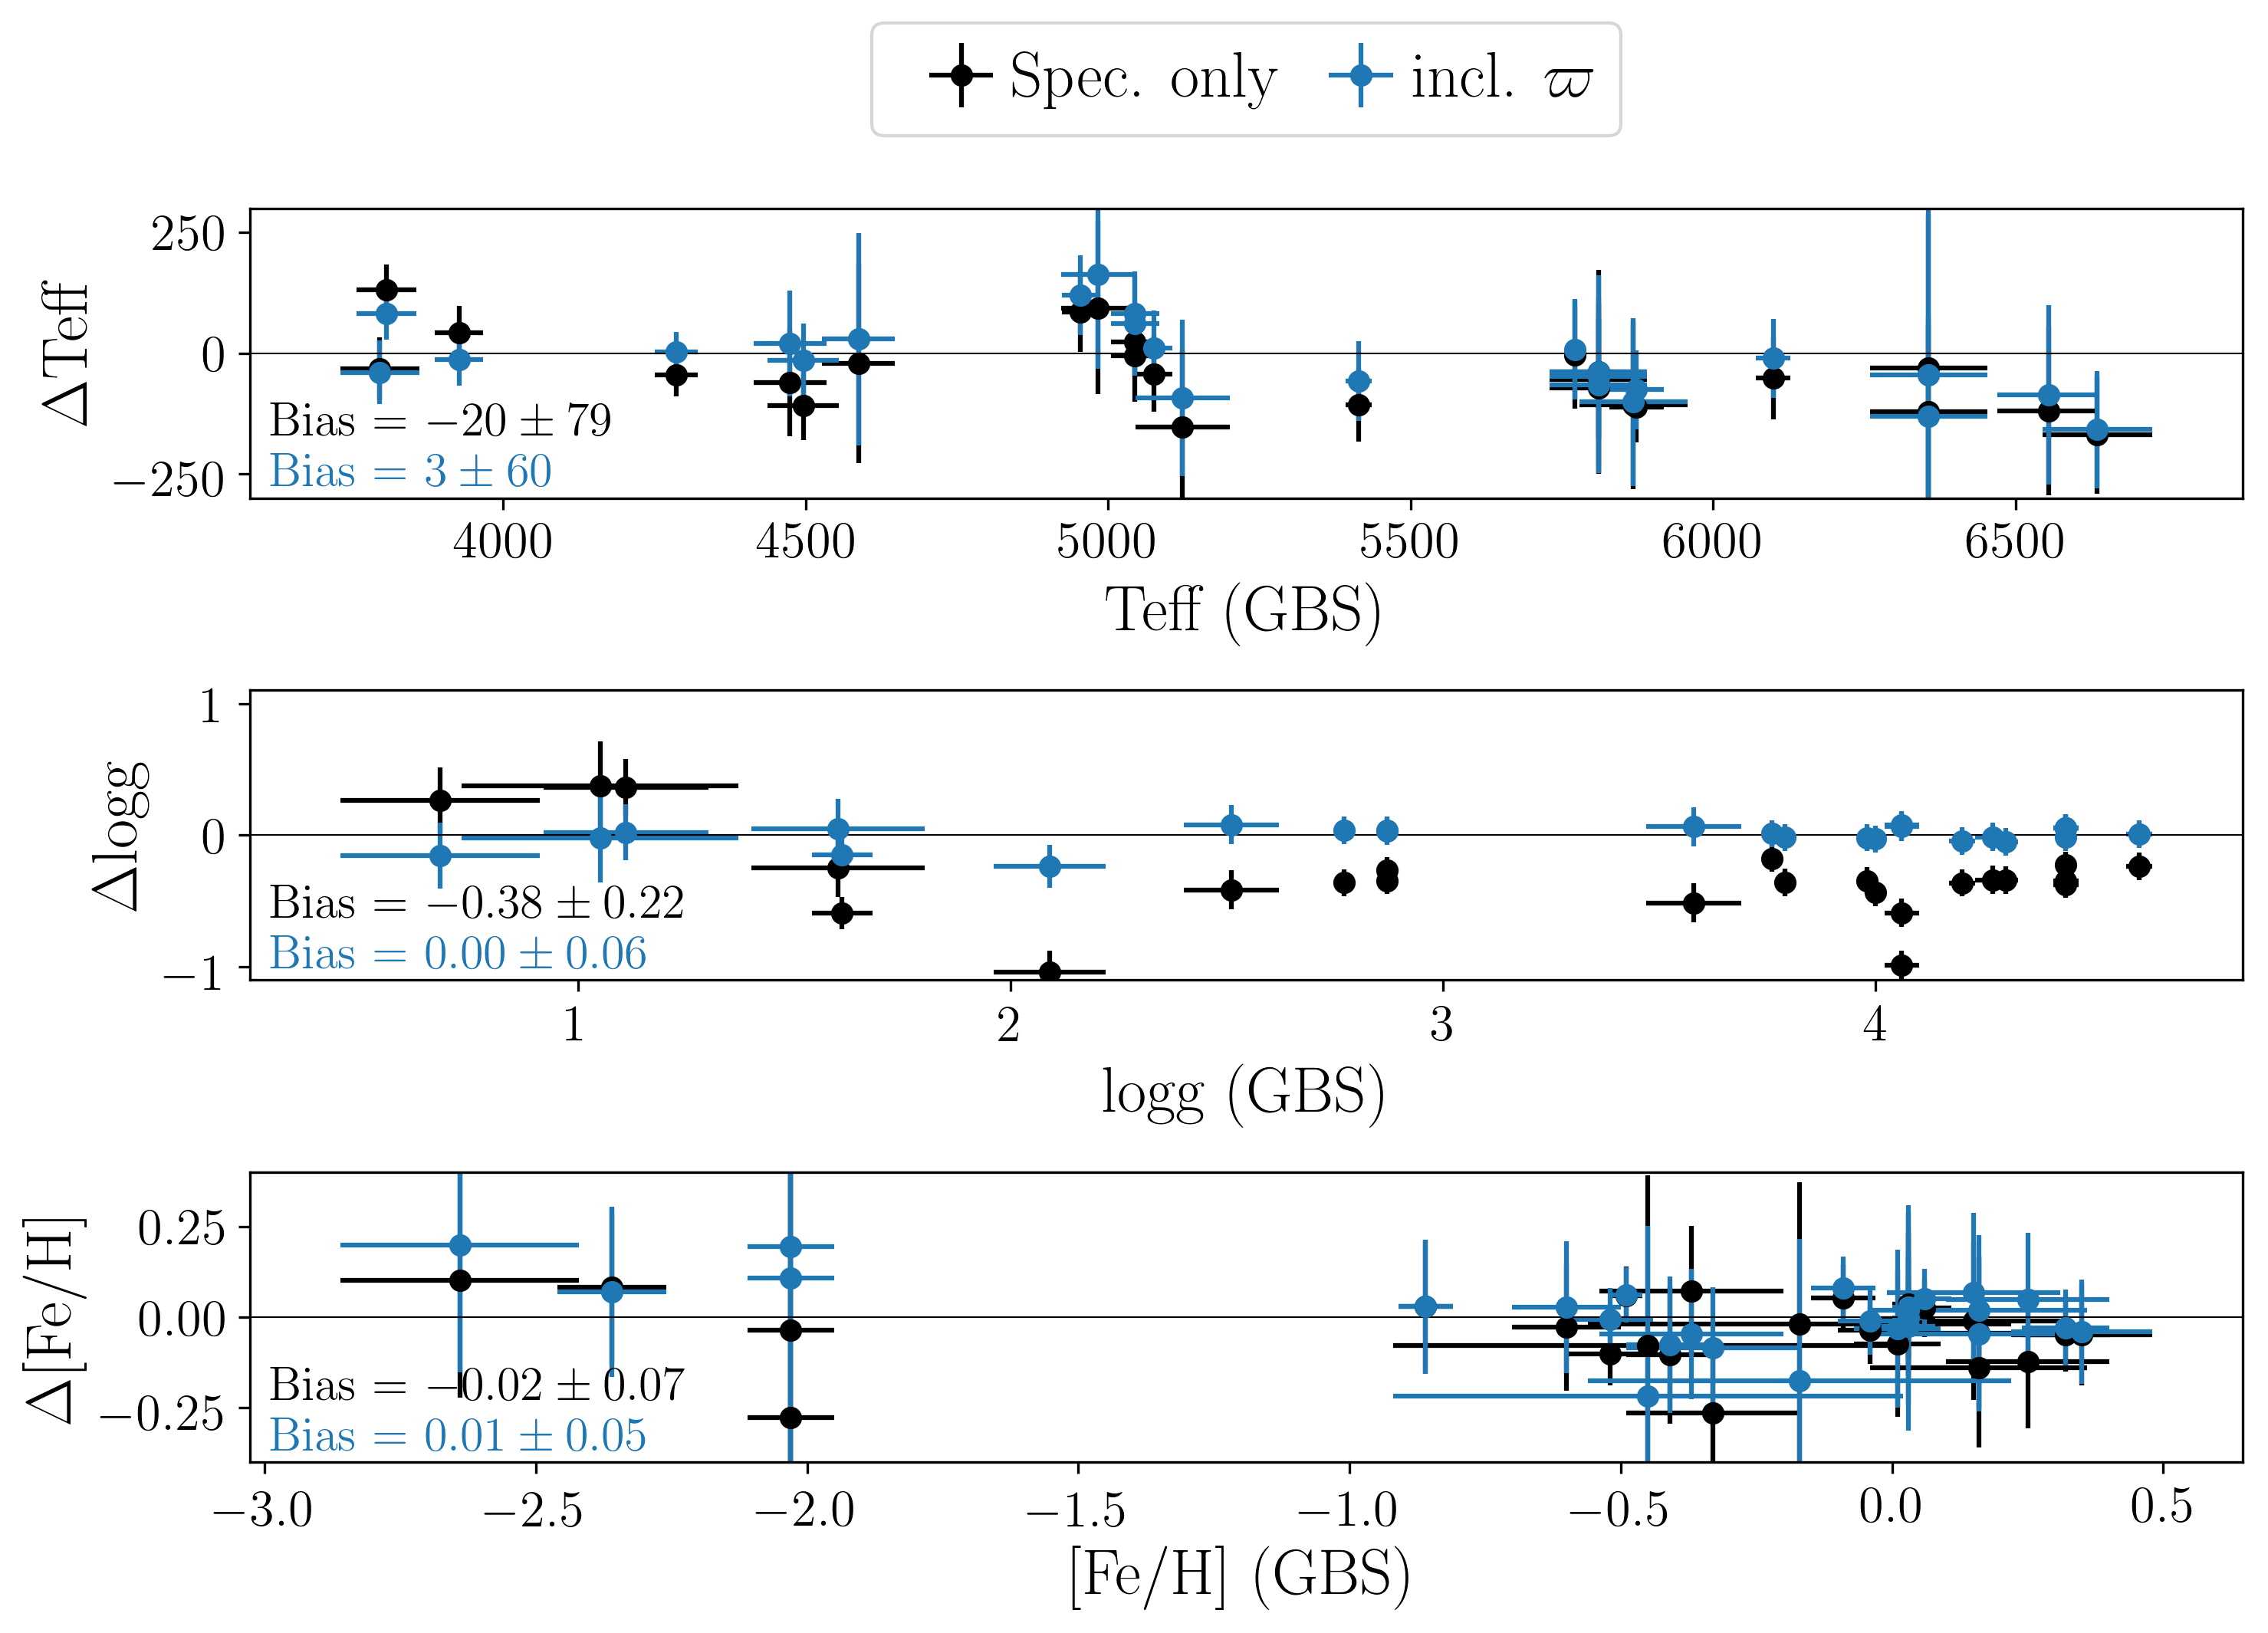
\includegraphics[width=\textwidth]{{Figures/gbs_performance_free_lbol}.png}
  \caption{Caption} 
  \label{fig:gbs_performance_free_lbol}
\end{figure*}

\subsubsection{Asteroseismic stars}

\begin{figure*}
 \centering
  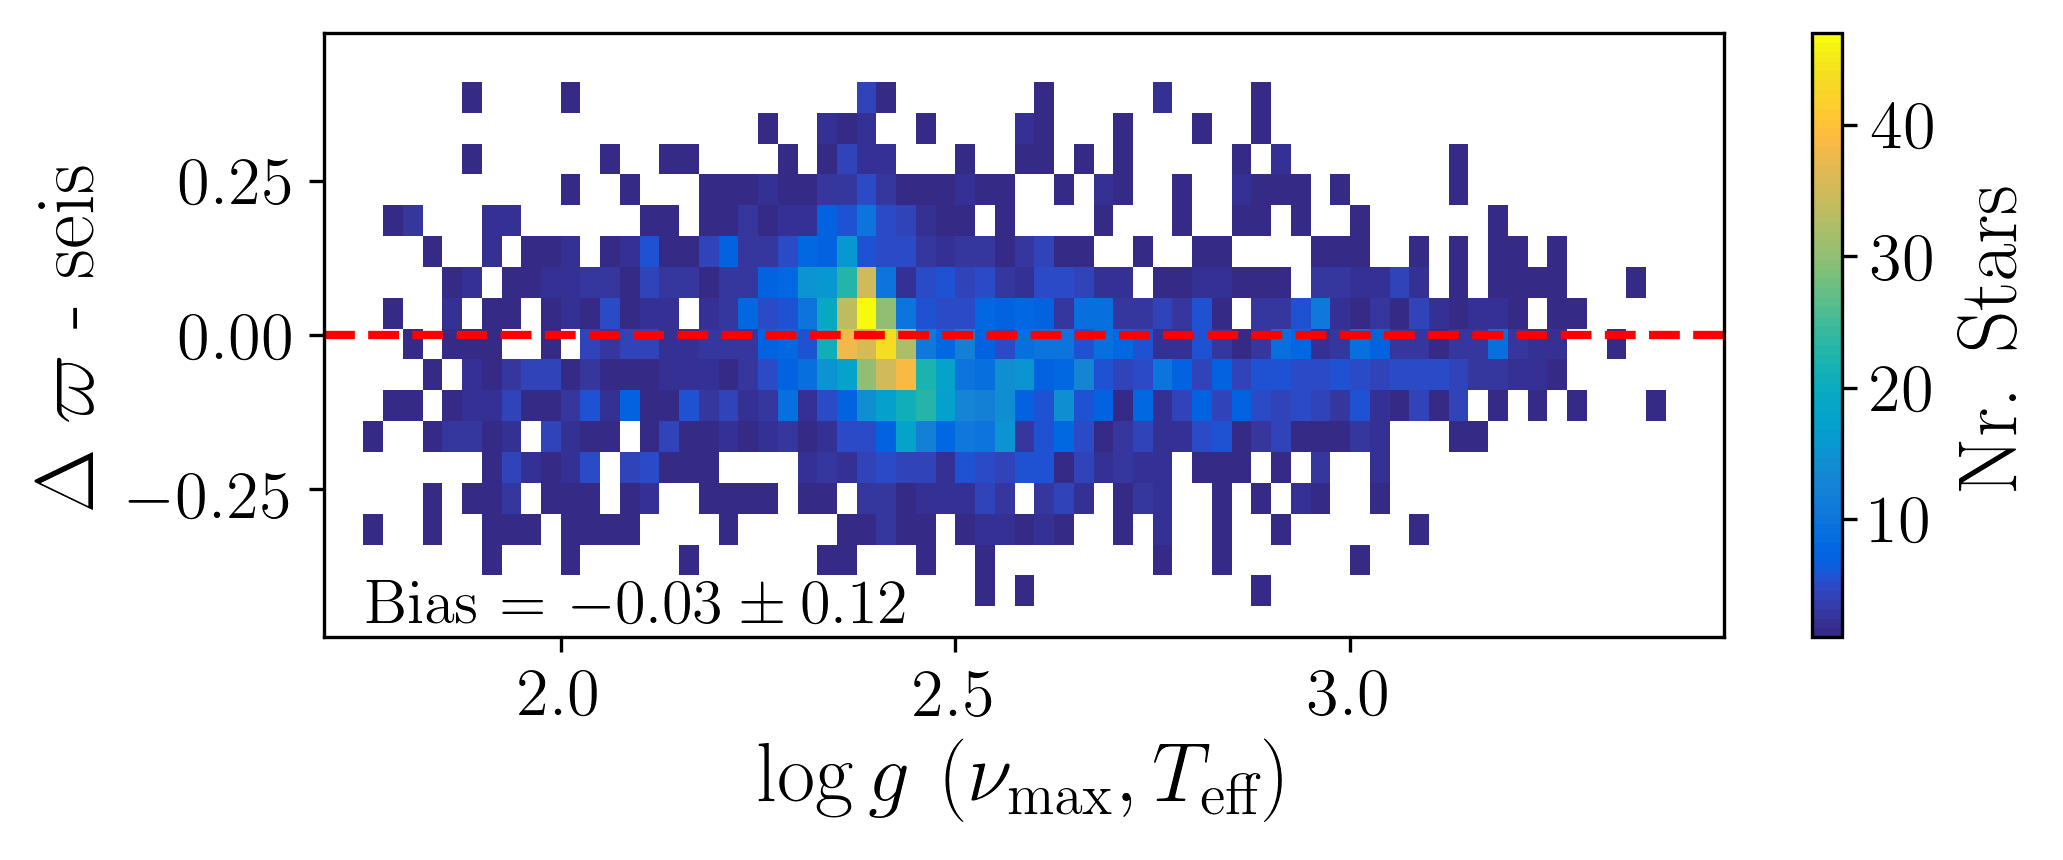
\includegraphics[width=0.49\textwidth]{{Figures/seismic_sample_delta_lbol}.png}
  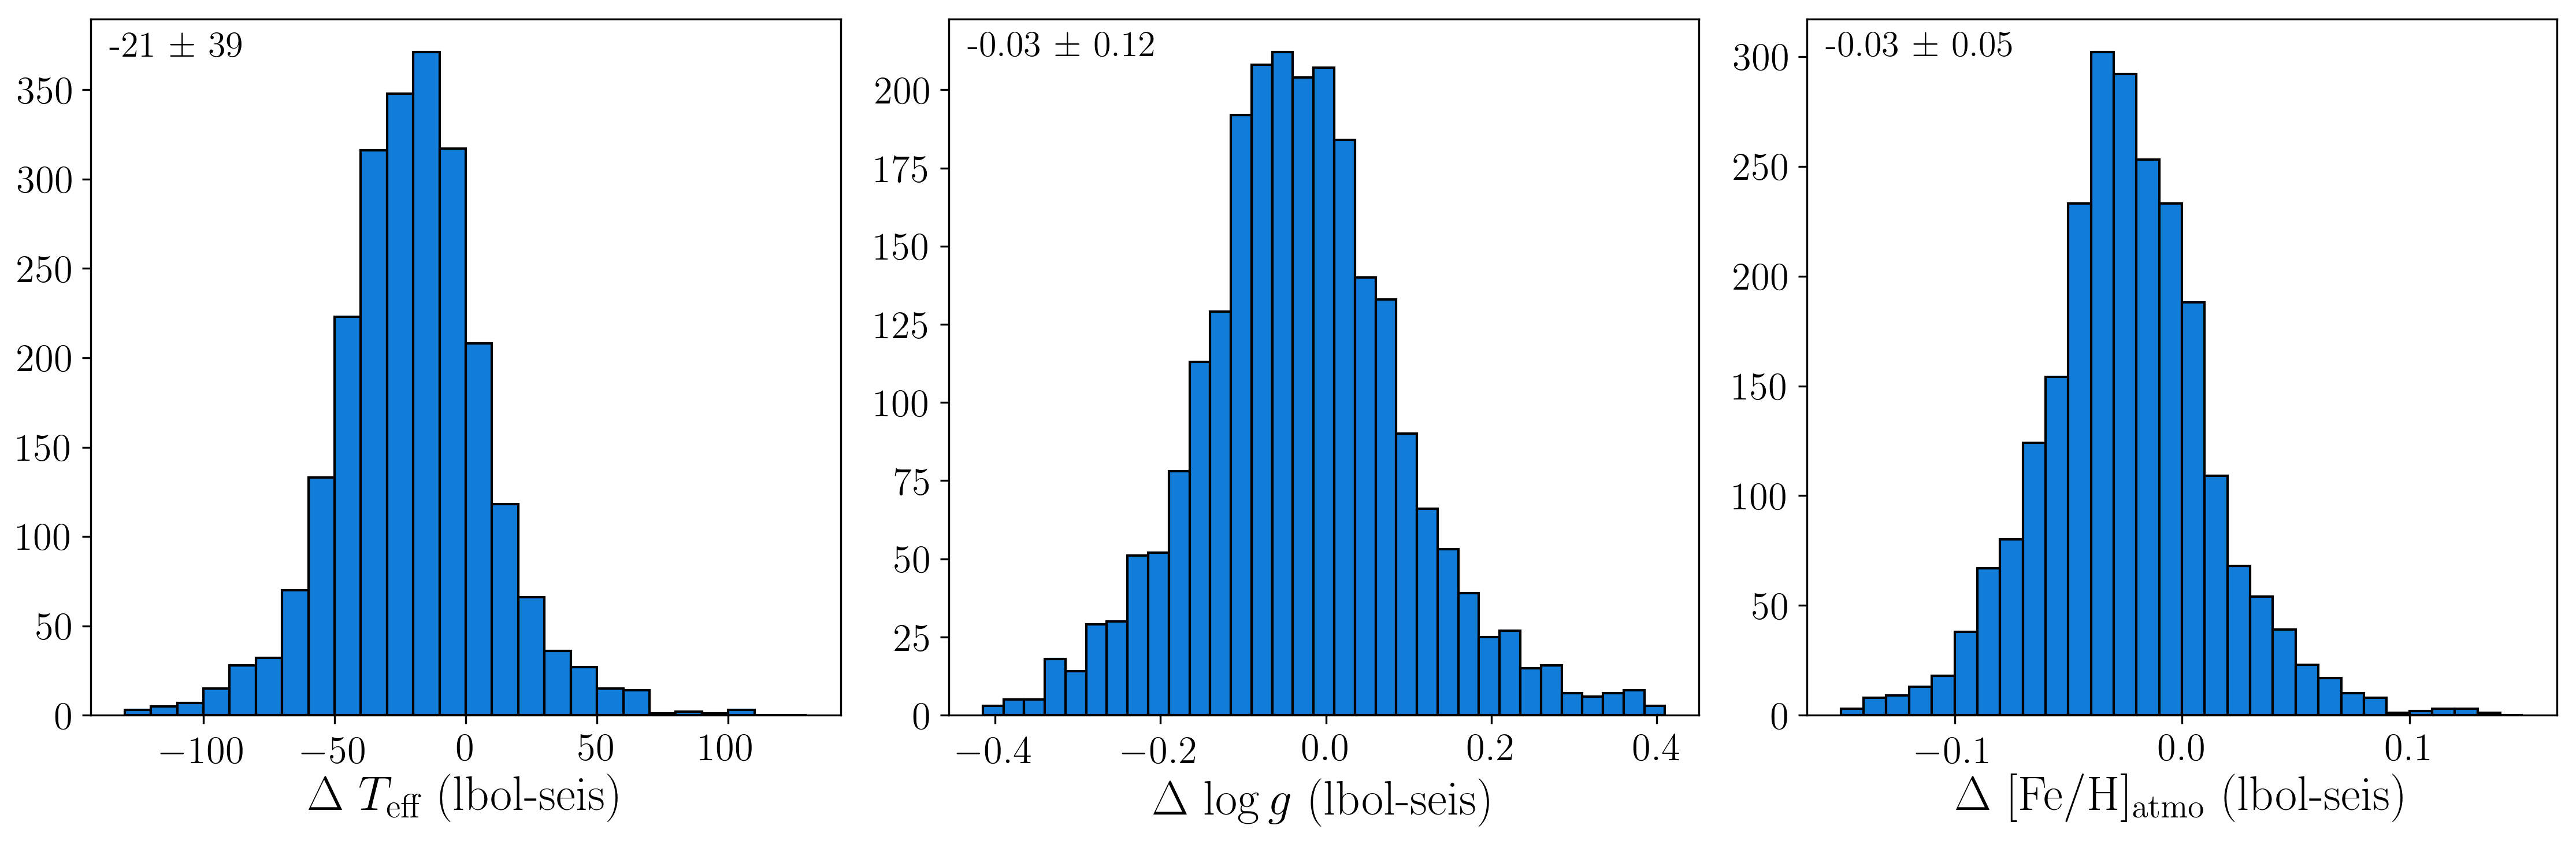
\includegraphics[width=0.49\textwidth]{{Figures/seis_setup_difference_lbol}.png}
  \caption{Caption} 
  \label{fig:seis_performance}
\end{figure*}

\subsubsection{Open and globular clusters}

\begin{figure*}
  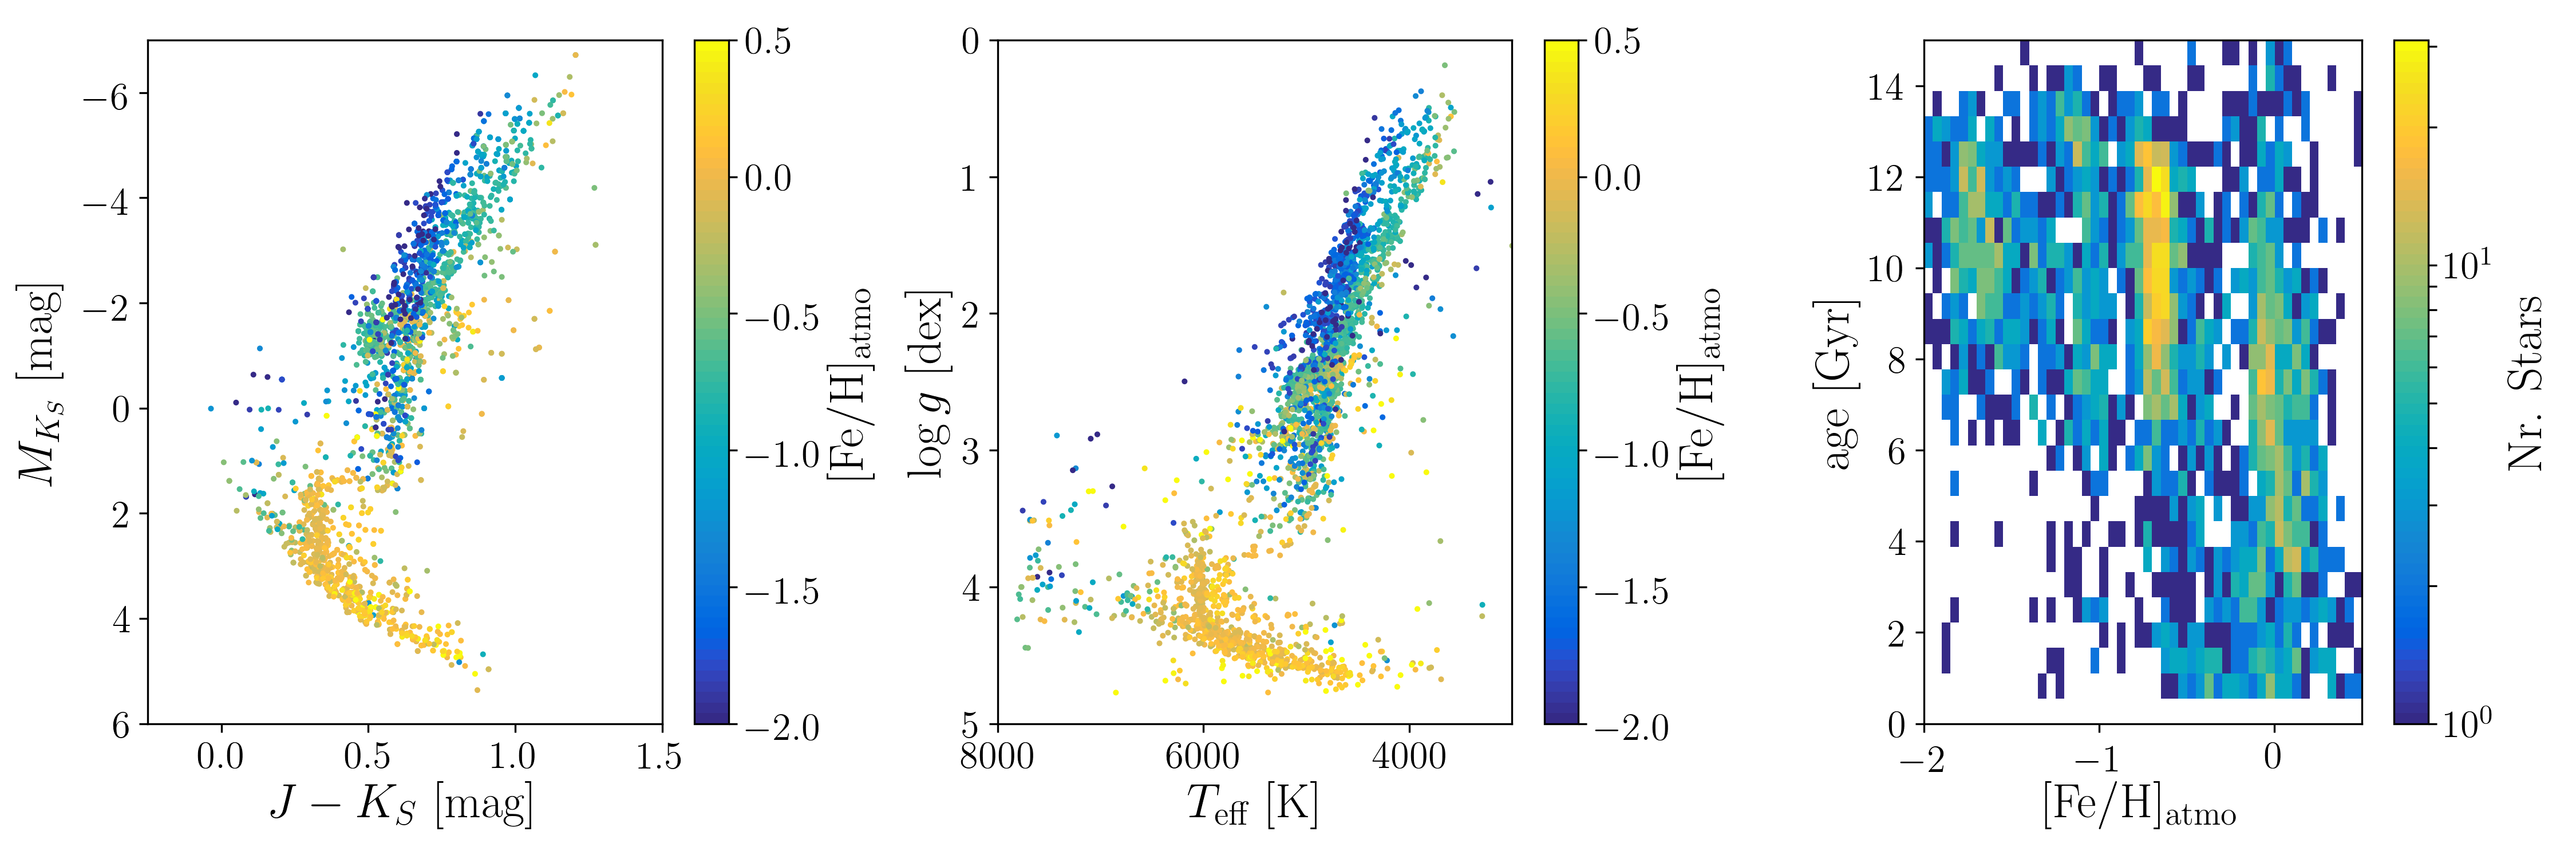
\includegraphics[width=\textwidth]{{Figures/CMD_Kiel_FehAge}.png}
  \caption{Caption} 
  \label{fig:CMD_Kiel_FehAge}
\end{figure*}

\subsection{Analysis step 3: Element abundances for the whole sample with \textit{Spectroscopy Made Easy}} \label{sec:analysis_step3}

\subsubsection{From a line-by-line analysis to the final element abundance}


\subsubsection{Abundance zeropoints}

\begin{figure*}
  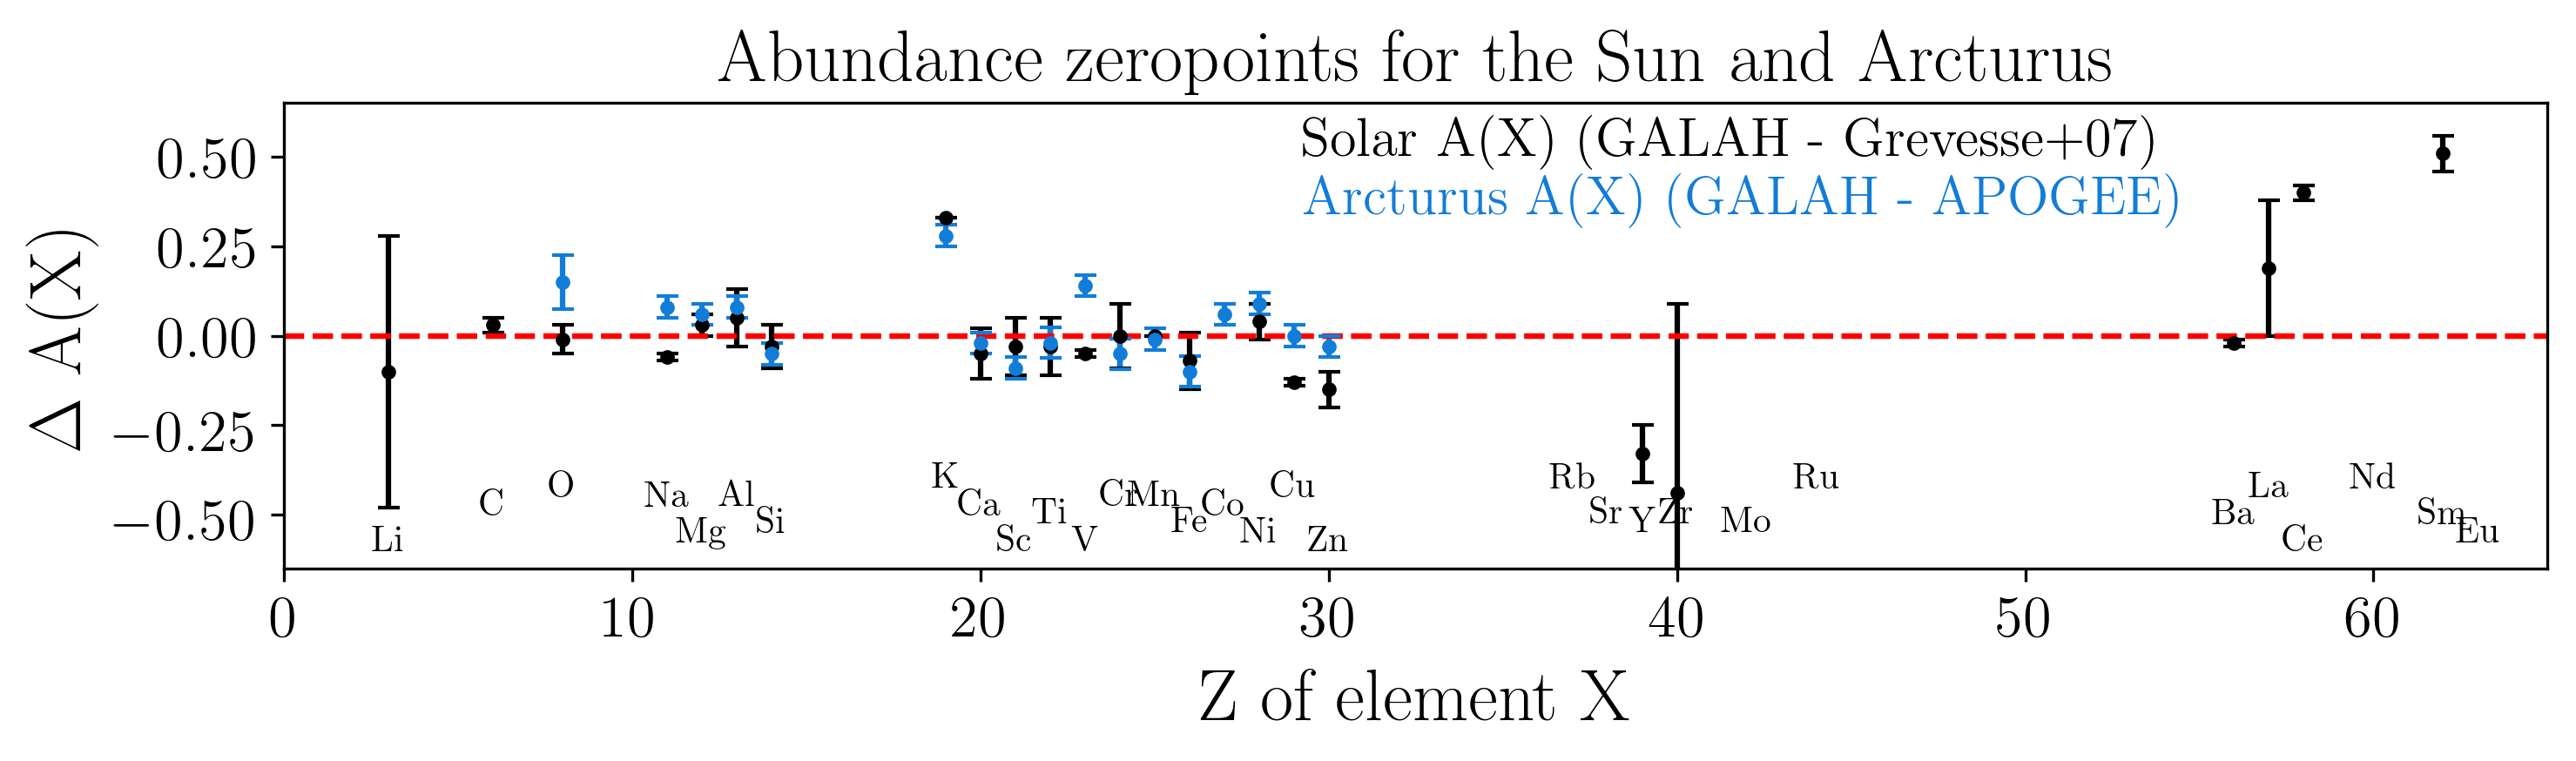
\includegraphics[width=\textwidth]{{Figures/abundance_zeropoints}.pdf}
  \caption{Caption} 
  \label{fig:abundance_zeropoints}
\end{figure*}

\subsection{Analysis step 4: Validation and flagging of element abundances} \label{sec:analysis_step4}

\subsection{Value added catalogs}

\subsubsection{Dynamics}

\begin{figure*}
  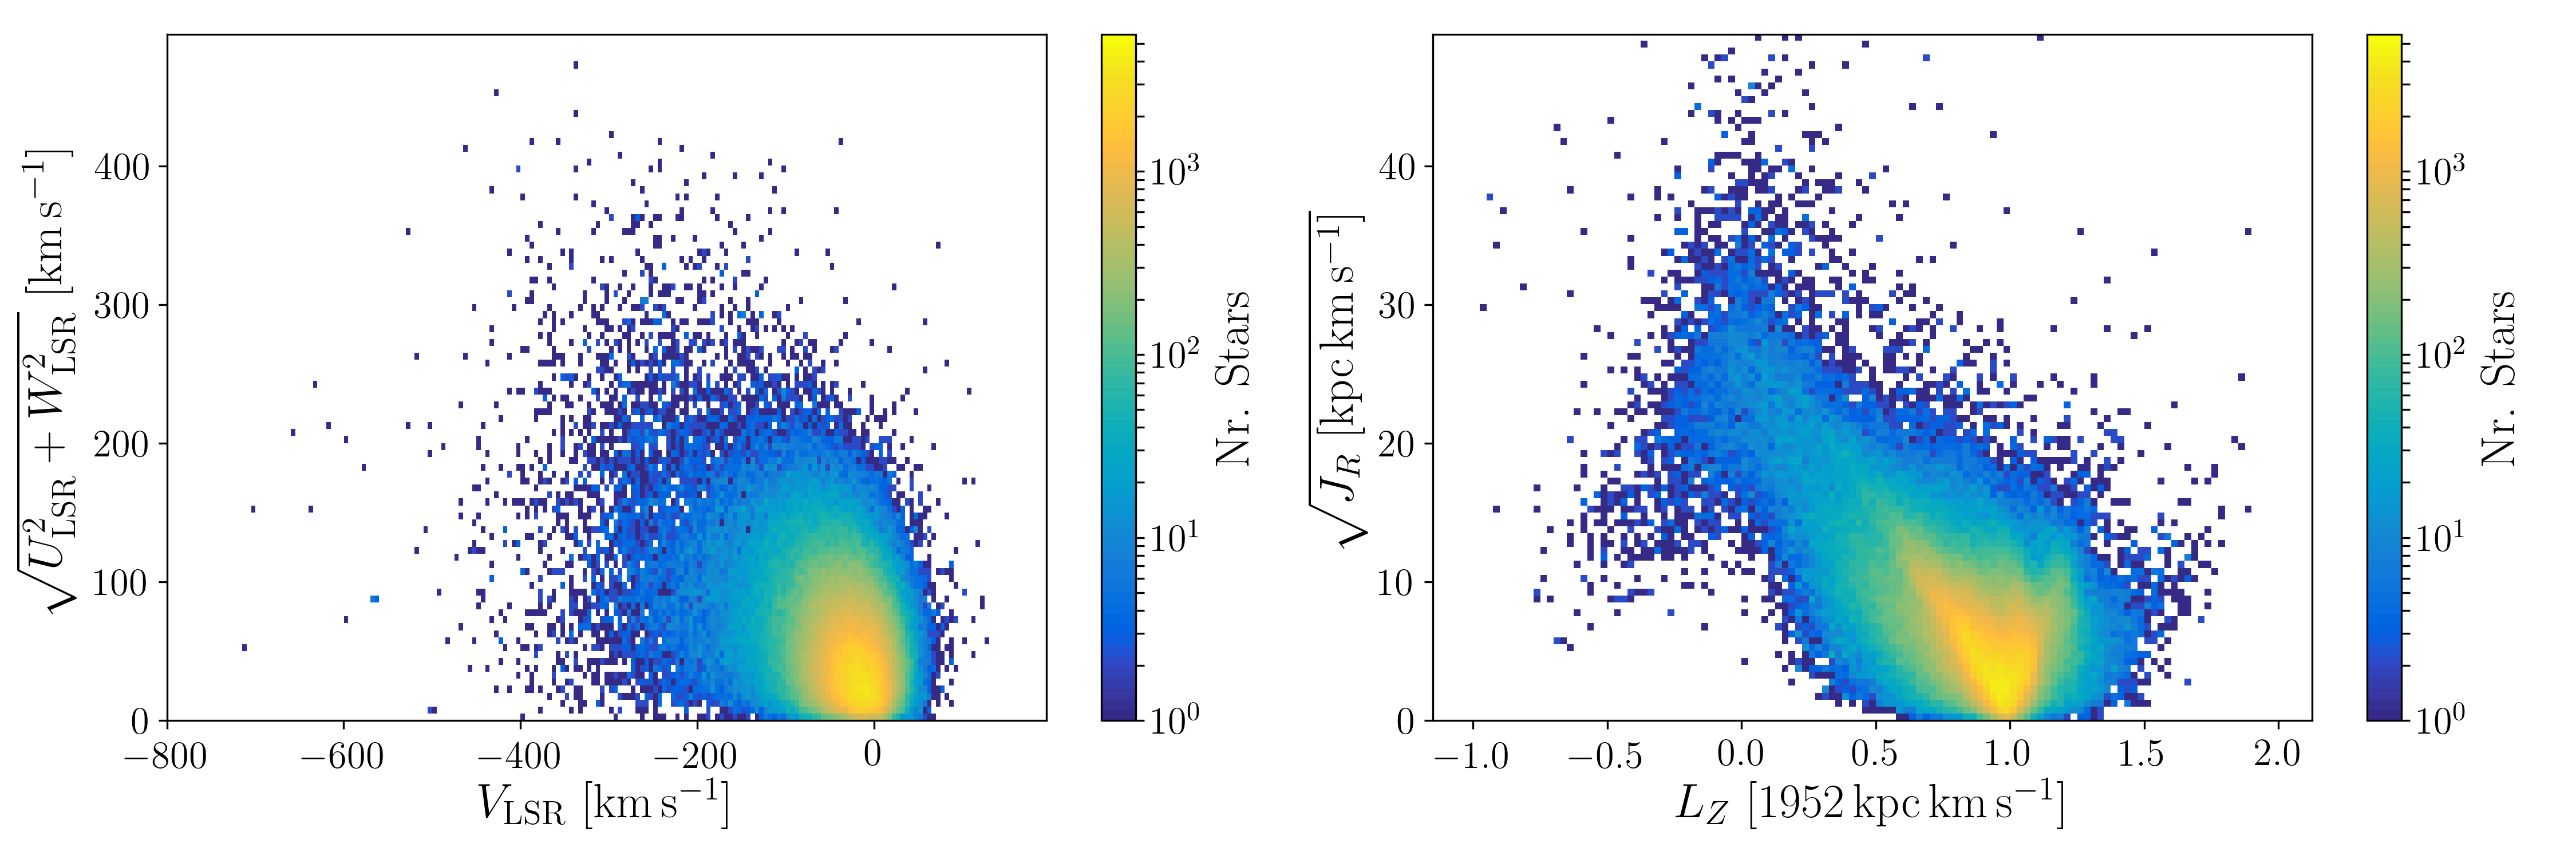
\includegraphics[width=\textwidth]{{Figures/action_overview_clean_all}.png}
  \caption{Caption} 
  \label{fig:action_overview_clean_all}
\end{figure*}



%\newpage
%________________________________________________________________
\section{Data catalog} \label{sec:catalog}

%\newpage
%________________________________________________________________
\section{Conclusions} \label{sec:conclusions}


%________________________________________________________________
\section*{Acknowledgements}
Based on data acquired through the Australian Astronomical Observatory, under programmes: A/2013B/13 (The GALAH pilot survey); A/2014A/25, A/2015A/19, A2017A/18 (The GALAH survey). We acknowledge the traditional owners of the land on which the AAT stands, the Gamilaraay people, and pay our respects to elders past and present.

The following software and programming languages made this research possible: \textsc{IRAF} \citep{Tody1986,Tody1993}, \textsc{configure} \citep{Miszalski2006}; Python (versions 2.7 \& 3.6); Astropy \citep[version 2.0;][]{Robitaille2013,PriceWhelan2018}, a community-developed core Python package for Astronomy; pandas \citep[version 0.20.2;][]{McKinney2011}; \textsc{topcat} \citep[version 4.4;][]{Taylor2005}; \textsc{galpy} \citep[version 1.3;][]{Bovy2015}. This research made use of APLpy, an open-source plotting package for Python \citep{Robitaille2012}. This research has made use of the VizieR catalogue access tool, CDS, Strasbourg, France. The original description of the VizieR service was published in A\&AS 143, 23.

This work has made use of data from the European Space Agency (ESA) mission {\it Gaia} (\url{http://www.cosmos.esa.int/gaia}), processed by the {\it Gaia} Data Processing and Analysis Consortium (DPAC, \url{http://www.cosmos.esa.int/web/gaia/dpac/consortium}). Funding for the DPAC has been provided by national institutions, in particular the institutions participating in the {\it Gaia} Multilateral Agreement.

SB acknowledges funds from the Alexander von Humboldt Foundation in the framework of the Sofja Kovalevskaja Award endowed by the Federal Ministry of Education and Research. SB acknowledges travel support from Universities Australia and Deutsche Akademische Austauschdienst. 

Parts of this research were conducted by the Australian Research Council Centre of Excellence for All Sky Astrophysics in 3 Dimensions (ASTRO 3D), through project number CE170100013. 

Parts of the computations were performed on resources provided by the MPCDF supercomputing facilities in Garching.

%%%%%%%%%%%%%%%%%%%%%%%%%%%%%%%%%%%%%%%%%%%%%%%%%%

%%%%%%%%%%%%%%%%%%%% REFERENCES %%%%%%%%%%%%%%%%%%

% The best way to enter references is to use BibTeX:

\bibliographystyle{mnras}
\bibliography{bib} % if your bibtex file is called example.bib

%%%%%%%%%%%%%%%%%%%%%%%%%%%%%%%%%%%%%%%%%%%%%%%%%%

\newpage
\noindent \rule{8.5cm}{1pt}

\noindent
% List of institutions
%$^{1}$Max Planck Institute  for Astronomy (MPIA), Koenigstuhl 17, 69117 Heidelberg, Germany\\
%$^{2}$Fellow of the International Max Planck Research School for Astronomy \& Cosmic Physics at the University of Heidelberg, Germany\\

%%%%%%%%%%%%%%%%% APPENDICES %%%%%%%%%%%%%%%%%%%%%

%\appendix

%%%%%%%%%%%%%%%%%%%%%%%%%%%%%%%%%%%%%%%%%%%%%%%%%%


% Don't change these lines
\bsp	% typesetting comment
\label{lastpage}
\end{document}


%%%%%%%%%%%%%%%%%%%%%%%%%%%%%%%%%%%%%%%%%%%%%%%%%%
%%%%%%%%%%%%%%%%%%%%%%%%%%%%%%%%%%%%%%%%%%%%%%%%%%
%%%%%%%%%%%%%%%%%%%%%%%%%%%%%%%%%%%%%%%%%%%%%%%%%%
%%%%%%%%%%%%%%%%%%%%%%%%%%%%%%%%%%%%%%%%%%%%%%%%%%